% !TeX spellcheck = sk_SK-Slovak
\documentclass[a4paper]{article}
\usepackage[slovak]{babel}
\usepackage[utf8]{inputenc}
\usepackage[T1]{fontenc}
\usepackage{a4wide}
\usepackage{amsmath}
\usepackage{amsfonts}
\usepackage{amssymb}
\usepackage{mathrsfs}
\usepackage[small,bf]{caption}
\usepackage{subcaption}
\usepackage{xcolor}
\usepackage{graphicx}
\usepackage{enumerate}
\usepackage{hyperref}
\usepackage{fancyvrb}
\usepackage{listings}
%\usepackage{lstautogobble}
\usepackage{stmaryrd}

\lstset{basicstyle=\ttfamily,
	mathescape=true,
	escapeinside=||%,
	%autogobble
}


\fvset{tabsize=4}


\pagestyle{empty}
\setlength{\parindent}{0pt}

\newenvironment{modenumerate}
{\enumerate\setupmodenumerate}
{\endenumerate}

\newif\ifmoditem
\newcommand{\setupmodenumerate}{%
	\global\moditemfalse
	\let\origmakelabel\makelabel
	\def\moditem##1{\global\moditemtrue\def\mesymbol{##1}\item}%
	\def\makelabel##1{%
		\origmakelabel{##1\ifmoditem\rlap{\mesymbol}\fi\enspace}%
		\global\moditemfalse}%
}

\makeatletter
\def\@seccntformat#1{%
	\expandafter\ifx\csname c@#1\endcsname\c@section\else
	\csname the#1\endcsname\quad
	\fi}
\makeatother

\begin{document} 
	
\pagenumbering{arabic}
\pagestyle{plain}

\begin{center}
	\sc\large
	Formálne metódy tvorby softvéru\\
	Domáca úloha 8
\end{center}

Autor: Marián Kravec


\section{1.)}

Sender\_A najkôr pošle správu akciou Send\_0 s bitom nula a prejde do stavov Sender\_B a Medium\_A, Sender\_B následne čaká až 5 časových jednotiek, či nedostane sa nie je možné spraviť akciu Ack\_rec\_0, medzitým Medium\_A môže správu stratiť alebo aktivovať Receiver\_B ktorý posiela správu do Receiver\_C ktorého úlohou je hlavne pri novej správe s opačným bitom správy kontrolovať, že predchádzajúca správa bola prijatá... v podstate, a do Medium\_B ktorý buď správu stratí alebo spolu so Sender\_B aktivuje Sender\_C a celý proces začína na novo s opačným bitom.

Skúmané vlastnosti:

\begin{figure}[!h]
	\centering
	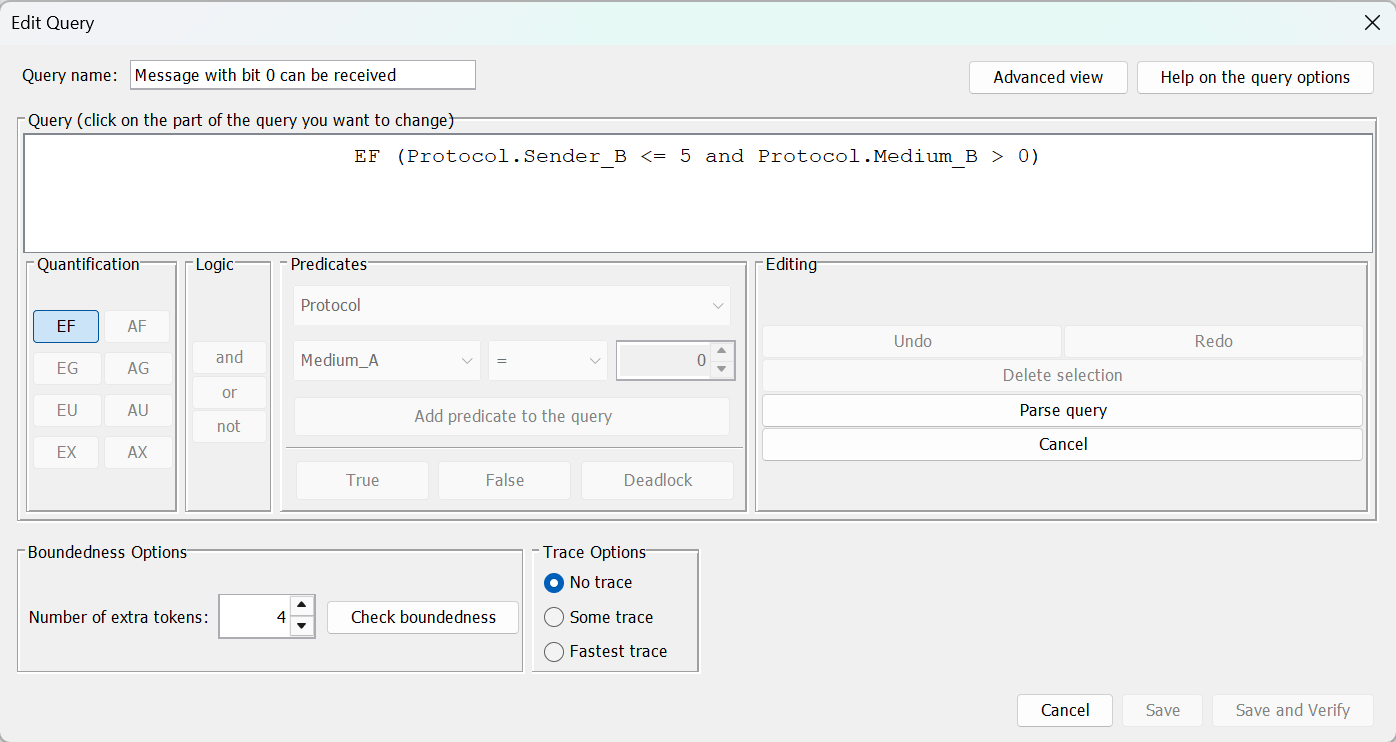
\includegraphics[width=0.7\textwidth]{Q1.png}
	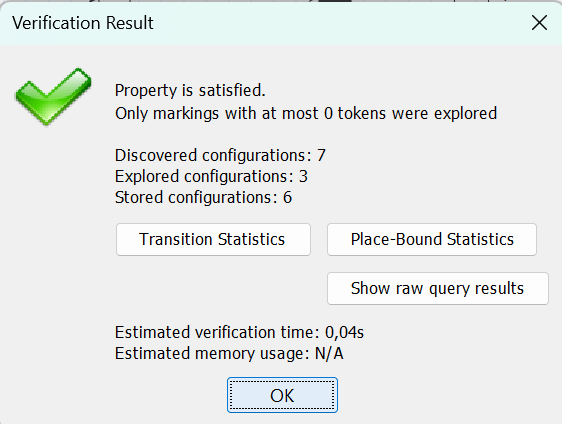
\includegraphics[width=0.3\textwidth]{R1.png}
	\caption{Správa 0 vie byť úspešne prijatá}
\end{figure}

\begin{figure}[!h]
	\centering
	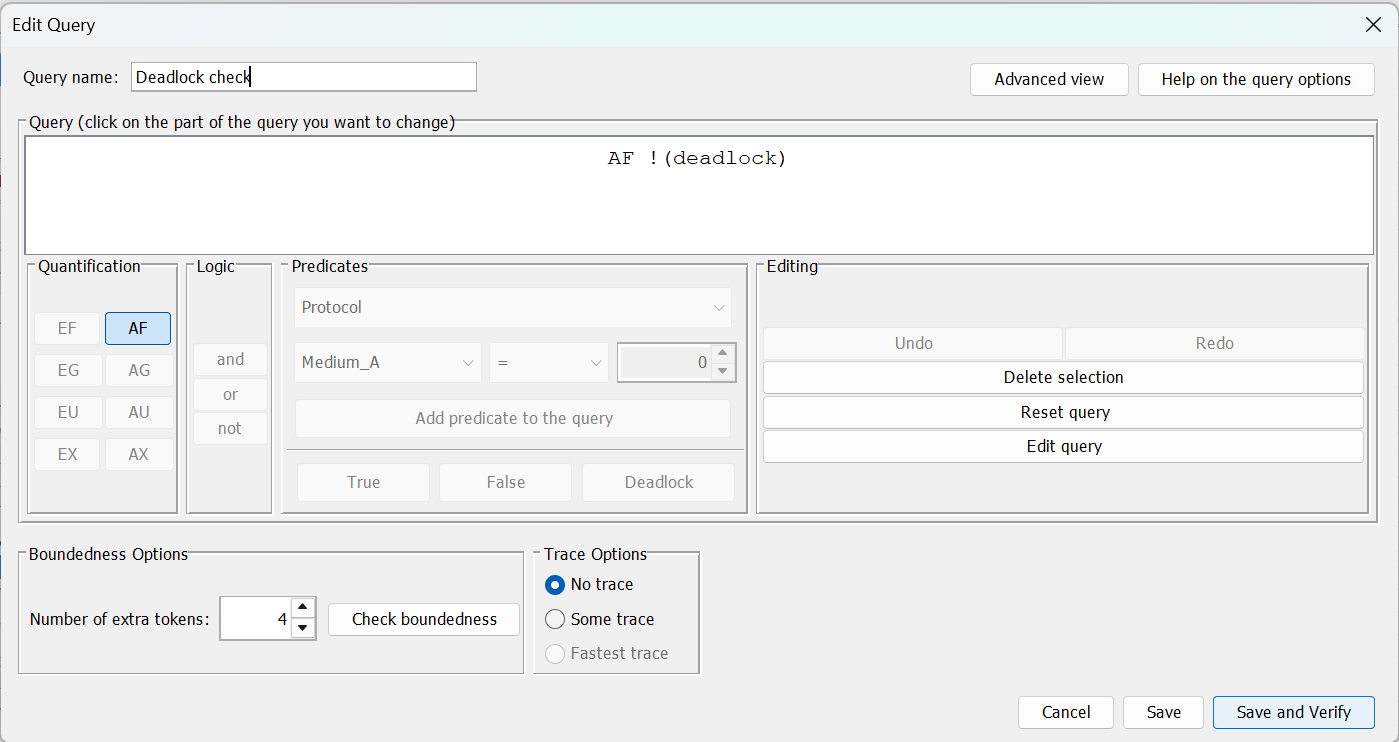
\includegraphics[width=0.7\textwidth]{Q2.png}
	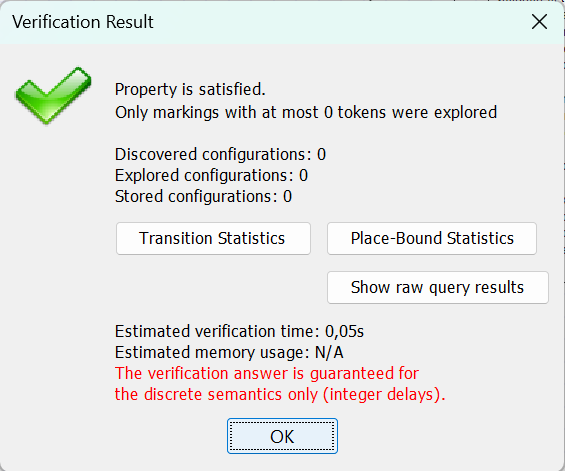
\includegraphics[width=0.3\textwidth]{R2.png}
	\caption{Nikdy nenastane deadlock}
\end{figure}

\begin{figure}[!h]
	\centering
	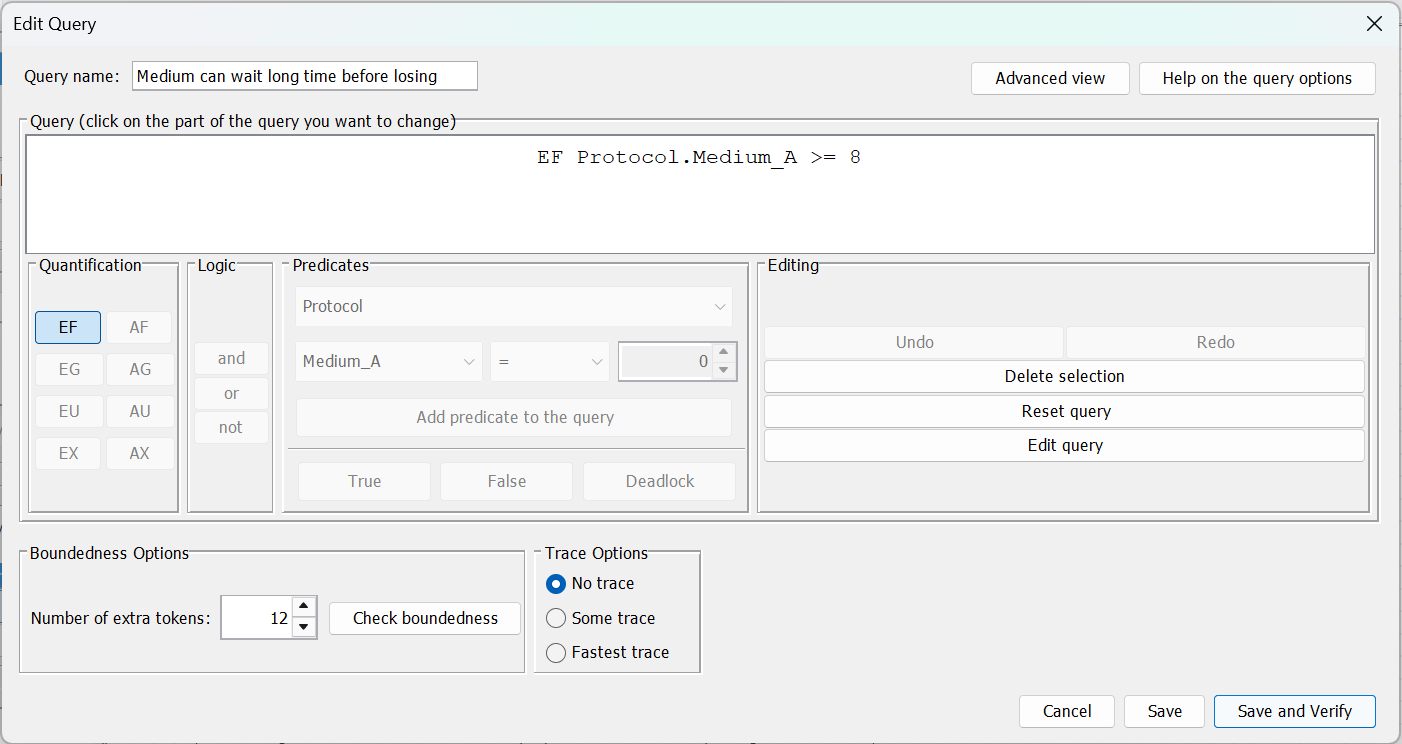
\includegraphics[width=0.7\textwidth]{Q3.png}
	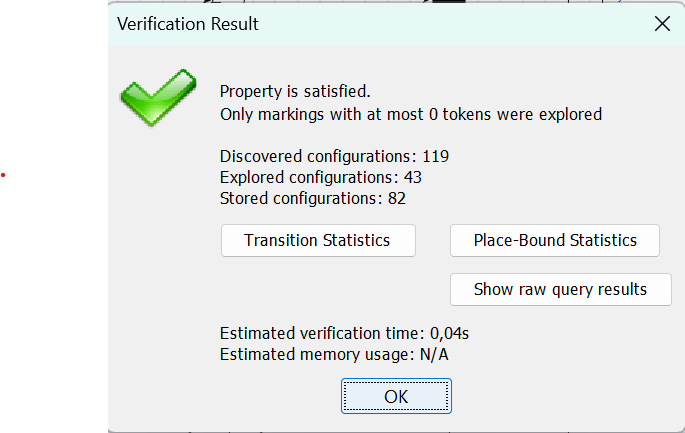
\includegraphics[width=0.3\textwidth]{R3.png}
	\caption{Medium vie držať správu dlhý čas predtým než ju stratí}
\end{figure}

\begin{figure}[!h]
	\centering
	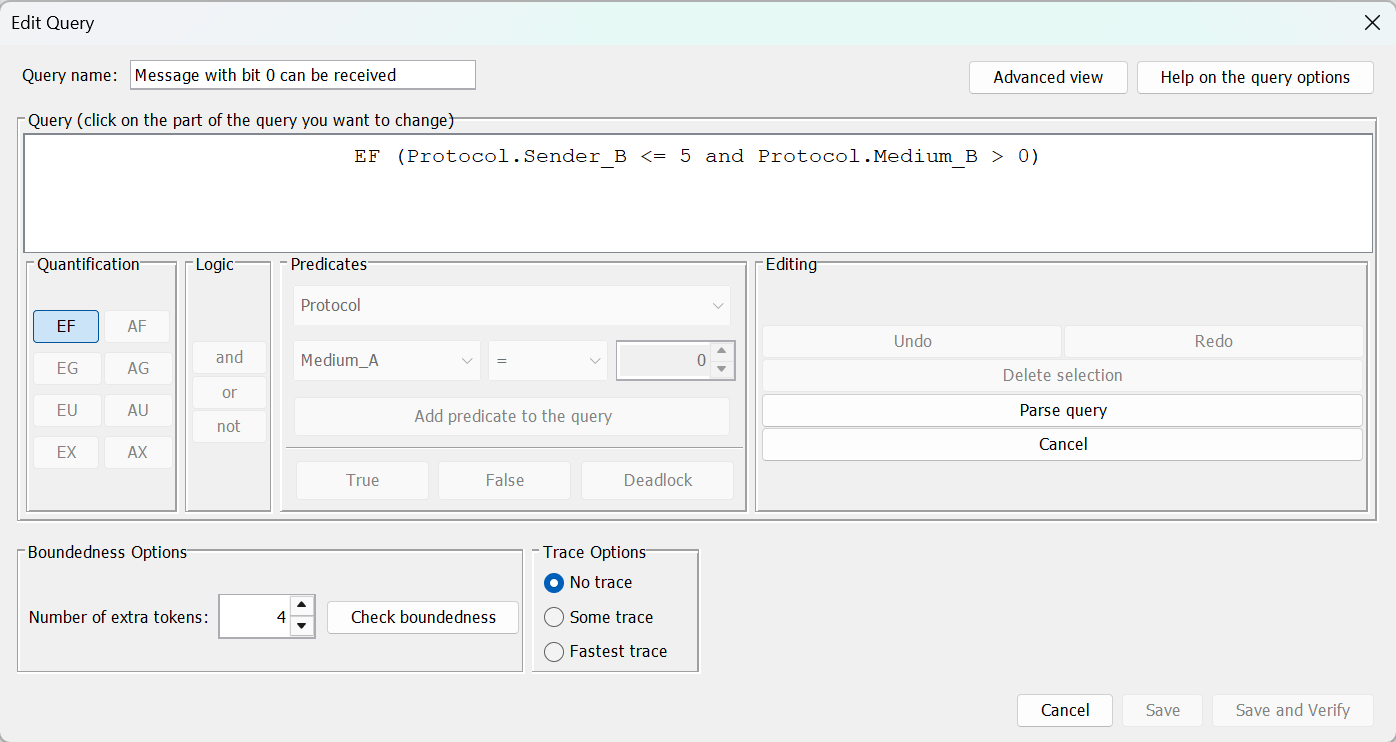
\includegraphics[width=0.7\textwidth]{Q1.png}
	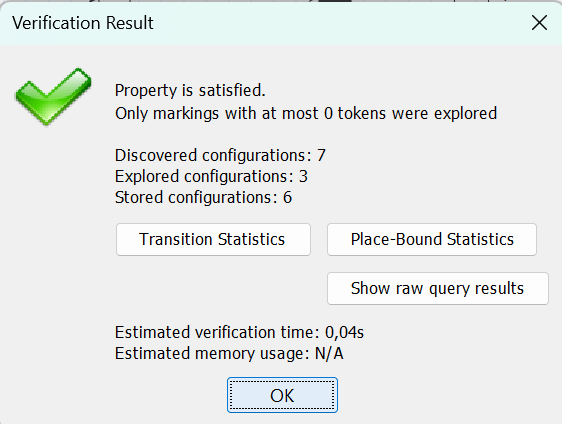
\includegraphics[width=0.3\textwidth]{R1.png}
	\caption{Správa 0 vie byť úspešne prijatá}
\end{figure}

\begin{figure}[!h]
	\centering
	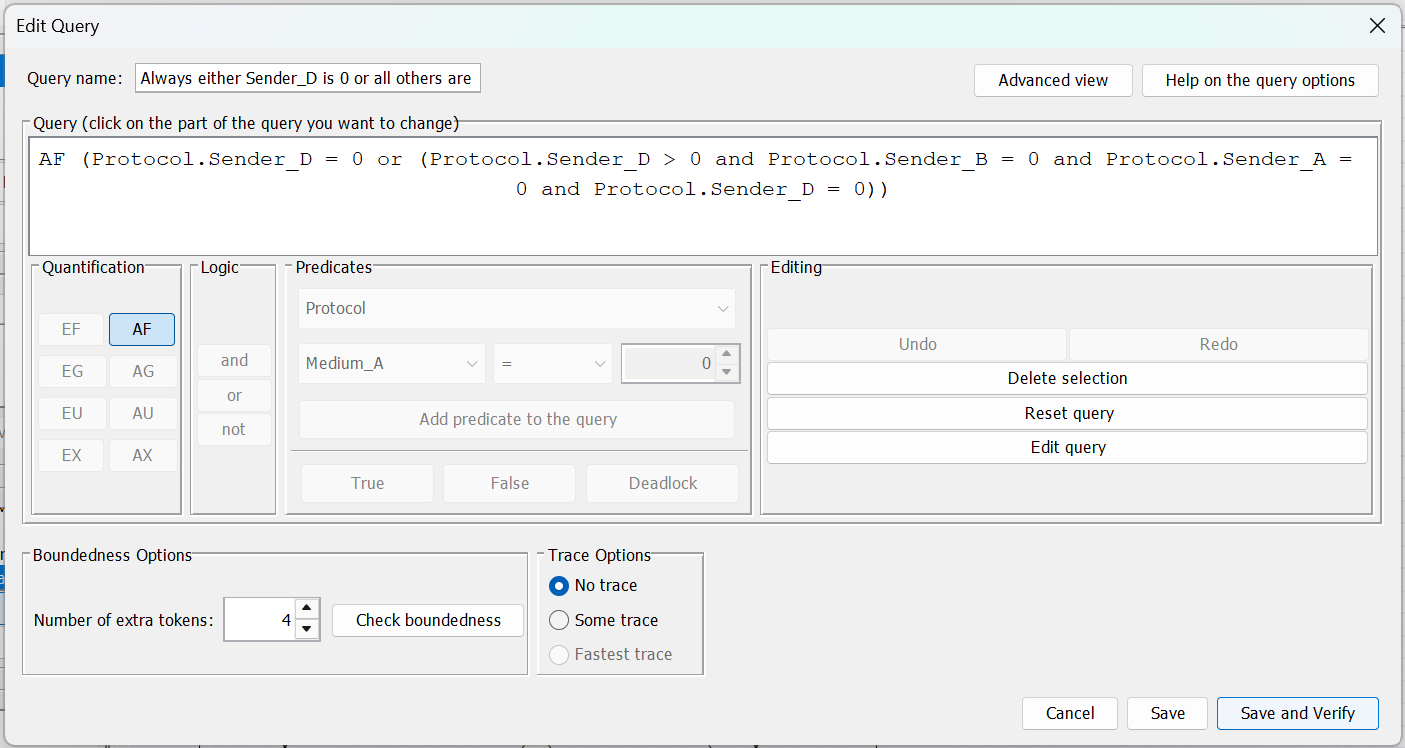
\includegraphics[width=0.7\textwidth]{Q4.png}
	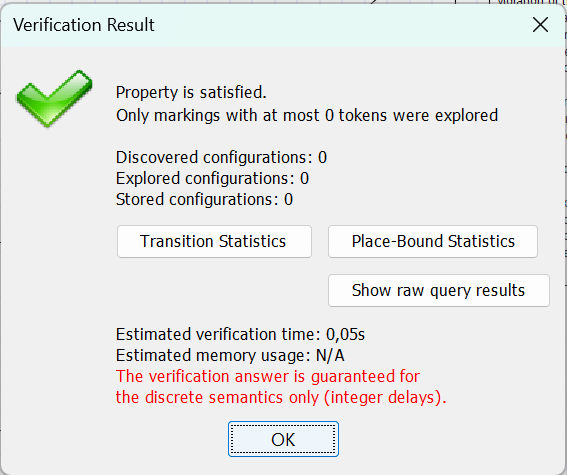
\includegraphics[width=0.3\textwidth]{R4.png}
	\caption{Vždy ak Sender\_D je nenulový všetci ostatný Senderi sú nulový}
\end{figure}
\newpage
.

\newpage
.

\newpage

\section{2.)}

Do modelu pridáme tester:

\begin{figure}[!h]
	\centering
	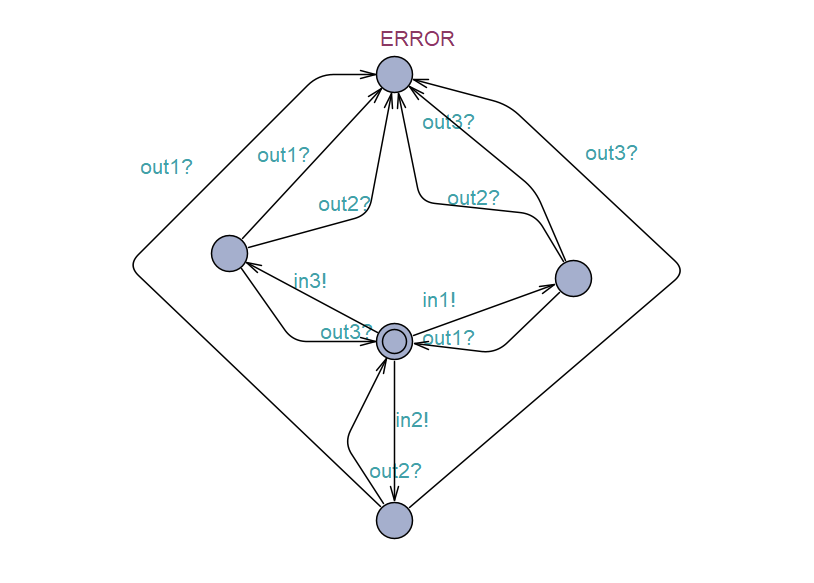
\includegraphics[width=1\textwidth]{tester.png}
	\caption{Tester}
\end{figure}

Súčasná verzia nevie dosiahnuť ERROR, čo je dobré.

\begin{figure}[!h]
	\centering
	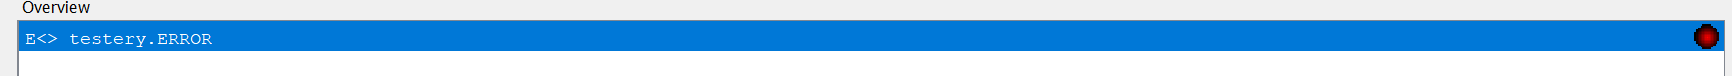
\includegraphics[width=1\textwidth]{R10.png}
	\caption{Dosiahnutie Erroru v pôvodnej verzii}
\end{figure}
\newpage

Pokazíme receiver tak, že pri bite 1 vždy pošle správu 2.

\begin{figure}[!h]
	\centering
	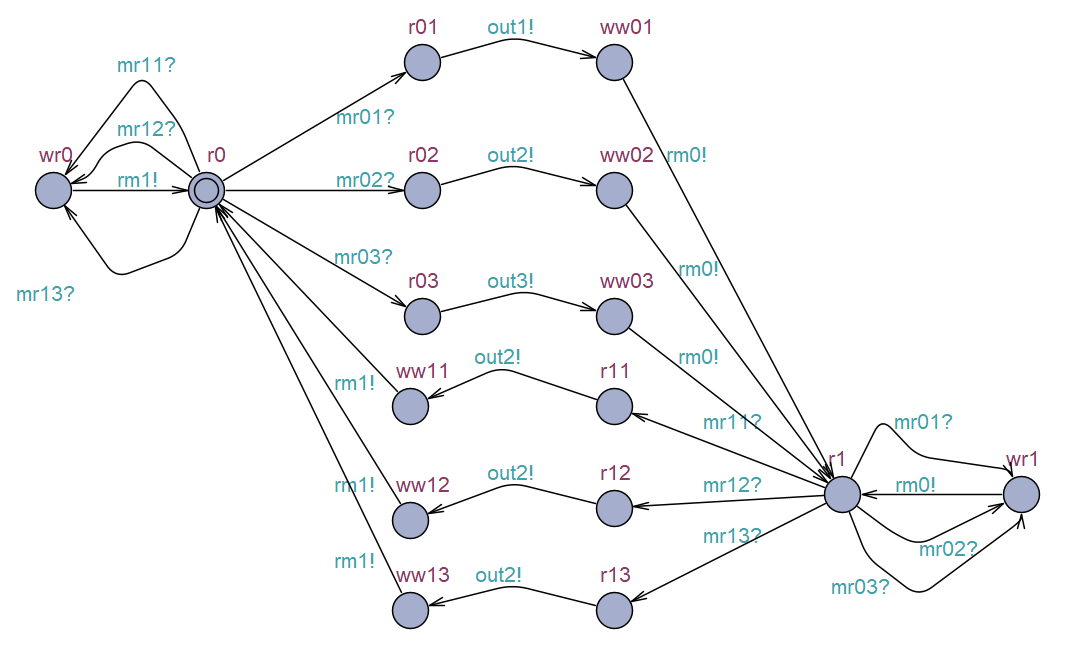
\includegraphics[width=1\textwidth]{rec.png}
	\caption{Modifikovaný receiver}
\end{figure}

Teraz je už ERROR dosiahnuteľný.

\begin{figure}[!h]
	\centering
	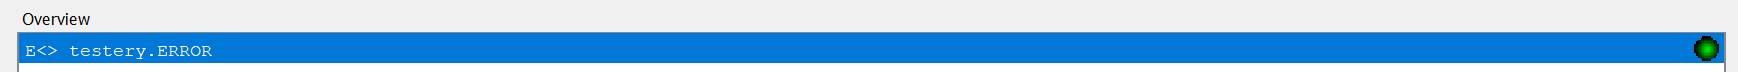
\includegraphics[width=1\textwidth]{R11.png}
	\caption{Dosiahnutie Erroru v modifikovanej verzii}
\end{figure}


\end{document}